\documentclass{scrartcl}

\usepackage{amssymb}
\usepackage{amsmath}
\usepackage{tikz}
\usetikzlibrary{calc}	%for centerarc

%via Kisiel, T. (1984). ``Diagrammatic Approach to Heidegger's Schematism of Existence.'' Philosophy Today 28(3), pp. 229-41	[p. 241]

\def\centerarc[#1](#2)(#3:#4:#5) %Syntax: [draw options](center)(initial angle:final angle:radius)
{ \draw[#1] ($(#2)+({#5*cos(#3)},{#5*sin(#3)})$) arc (#3:#4:#5); }

\begin{document}
	
	\hspace{-1.5cm}		%for centering
	%\begin{figure}
	%	\centering
	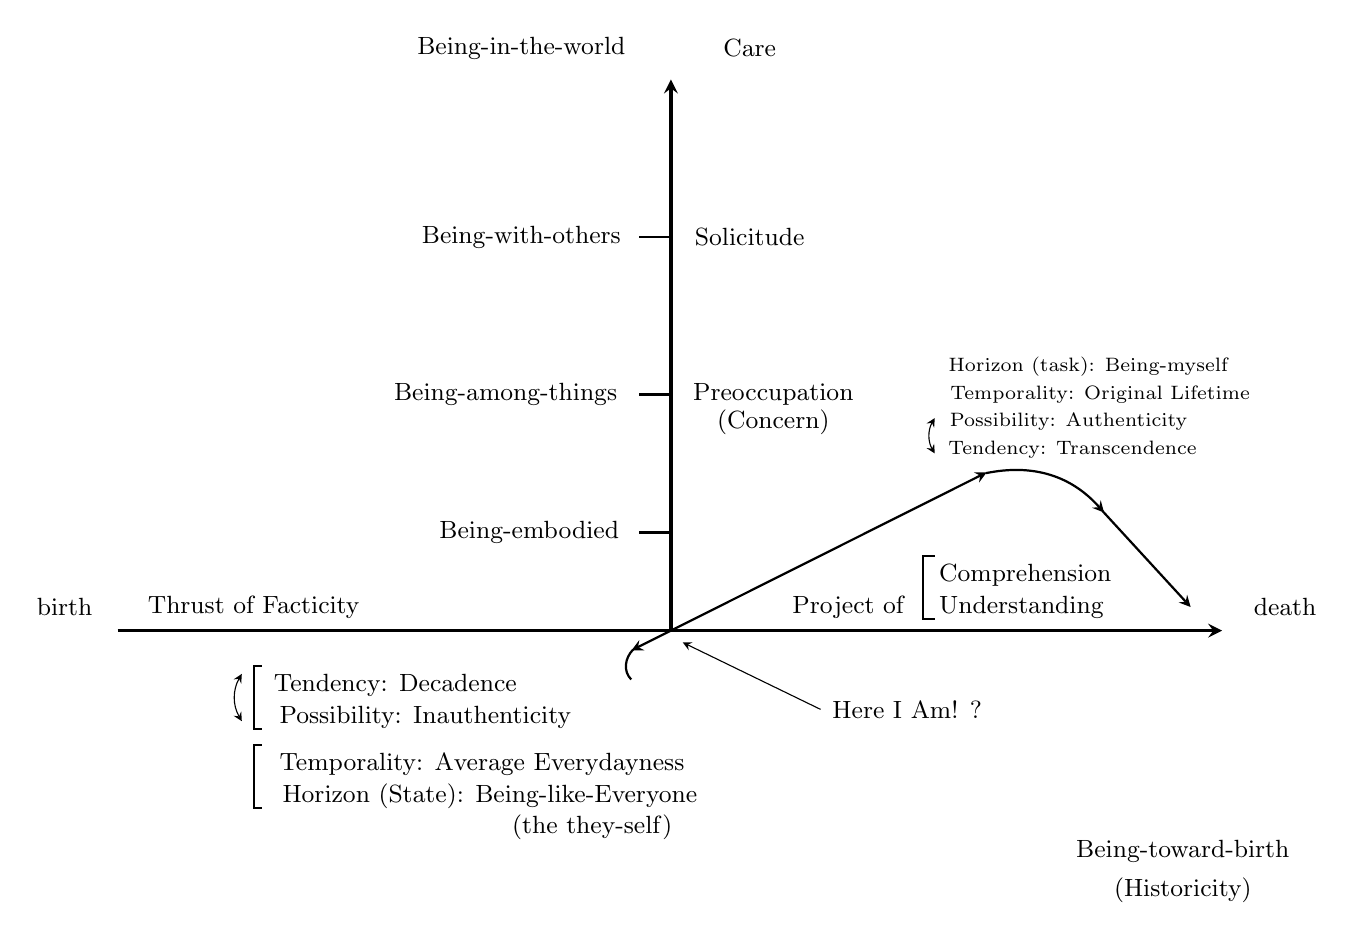
\begin{tikzpicture}
	%main arc
	\centerarc[->,>=stealth,ultra thick](0,0)(180:-20:7)	%big arc
	\draw[->,>=stealth,very thick] (-7.0275,0)--(7,0);		%x-axis
	\draw[->,>=stealth,very thick] (0,0)--(0,7);			%y-axis
		\draw[line width=1pt] (0,1.25)--(-0.4,1.25);		%tab on y-axis
		\draw[line width=1pt] (0,3)--(-0.4,3);
		\draw[line width=1pt] (0,5)--(-0.4,5);
	
	%upper labels
	\node at (-7.7,0.3)  {\small birth};
	\node at (-5.3,0.3)  {\small Thrust of Facticity};	
	%
	\node at (-1.9,7.4)	{\small Being-in-the-world};
	\node at (1,7.4)	{\small Care};
	\node at (-1.9,5)	{\small Being-with-others};
	\node at (1,5)		{\small Solicitude};
	\node at (-2.1,3)	{\small Being-among-things};
	\node at (1.3,3)	{\small Preoccupation};
	\node at (1.3,2.65) {\small (Concern)};
	\node at (-1.8,1.25){\small Being-embodied};
	%
	\node at (3,-1) {\small Here I Am! ?};
	\draw[->,>=stealth] (1.9,-1)--(0.15,-0.15);
	%
	\node at (2.25,0.3) {\small Project of};
	\draw[thick] (3.35,0.95)--(3.2,0.95)--(3.2,0.15)--(3.35,0.15);	%bracket
	\node at (4.5,0.7)  {\small Comprehension};
	\node at (4.45,0.3) {\small Understanding};
	%
	\node at (7.8,0.3)  {\small death};
	\node at (6.5,-2.8) {\small Being-toward-birth};
	\node at (6.5,-3.3) {\small (Historicity)};
	
	%lower labels (below axis)
	\draw[thick] (-5.2,-0.45)--(-5.3,-0.45)--(-5.3,-1.25)--(-5.2,-1.25);	%top bracket
	\draw[thick] (-5.2,-1.45)--(-5.3,-1.45)--(-5.3,-2.25)--(-5.2,-2.25);	%bottom bracket
	%
	\draw[<->,>=stealth] (-5.45,-0.55) to[bend right] (-5.45,-1.15);
	\node at  (-3.5,-0.7)  {\small Tendency: Decadence};
	\node at  (-3.12,-1.1) {\small Possibility: Inauthenticity};
	%
	\node at  (-2.4,-1.7) {\small Temporality: Average Everydayness};
	\node at  (-2.3,-2.1) {\small Horizon (State): Being-like-Everyone};
	\node at  (-1.0,-2.5) {\small (the they-self)};
	
	%labels above arrow thing
	\centerarc[line width=2.2pt,white](0,0)(18:30:7)
	\node at (5.3,3.35)  {\scriptsize Horizon (task): Being-myself};
	\node at (5.45,3) 	 {\scriptsize Temporality: Original Lifetime};
	\draw[<->,>=stealth] (3.35,2.7) to[bend right] (3.35,2.25);
	\node at (5.05,2.65) {\scriptsize Possibility: Authenticity};
	\node at (5.1,2.3)	 {\scriptsize Tendency: Transcendence};
	
	%weird arrow thing
	\centerarc[->,>=stealth,thick](0,0)(-47:120:0.8)
	\centerarc[->,>=stealth,thick](0,0)(-130:-45:0.8)
	\draw[thick] (-0.505,-0.62) to[out=135,in=225] (-0.48,-0.24);
	\draw[<->,>=stealth,thick] (-0.5,-0.25)--(4.01,2.01);
	\draw[->,>=stealth,thick] (4,2) to[bend left] (5.5,1.5);
	\draw[->,>=stealth,thick] (5.48,1.52)--(6.6,0.3);
	
	%\draw[help lines] (-9,-9) grid (9,9);
	\end{tikzpicture}
	%	\caption{Heidegger's Schematism of Existence (Kisiel, 1984)}
	%\end{figure}
	
\end{document}